\section{Numerical results}
\label{sec:numerics}

\subsection{Analysis of bias terms in synthetic data}

In this part, we simulate an example where geolocation is used to construct proxy for race. We use this example to demonstrate different sources of overestimation and underestimation bias of the weighted estimator and the thresholded estimator.

\paragraph{Experimental setup}
We consider race as the unknown protected attribute $A$ with $A = a$ being the advantaged racial group and $A = b$ being the disadvantaged racial group. Suppose there are three different neighborhoods ($Z = z_1, z_2, z_3$) where the proportions of people belonging to the advantaged group are $0.2, 0.5, 0.8$ respectively. These proportions are in turn the race proxy probabilities. For example, all people who live in the neighborhood $z_1$ are assigned with $(\pr (A = a \mid Z = z_1) = 0.2, \pr (A = b \mid Z = z_1)  = 0.8)$ as their race proxy. If we apply the thresholded estimation rule with $q = 0.75$, the estimated races for people living in neighborhoods tracts are:
\begin{center}
\begin{tabular}{|c||c|c|c|}
\hline
 & $Z=z_{1}$ & $Z=z_{2}$ & $Z=z_{3}$\tabularnewline
\hline
\hline
$\hat{A}$ & $b$ & NA & $a$\tabularnewline
\hline
\end{tabular}
\end{center}
% \begin{equation*} \textstyle
% \hat{A} =\left\{
% \begin{aligned}
% &a, \  Z = z_1, \\
% &b, \ Z = z_3, \\
% &\text{NA}, \ Z = z_2.
% \end{aligned}
% \right.
% \end{equation*}
We assume that geolocation is strongly correlated with people's income $X$: $\expect (X \mid Z = z_1) < \expect (X \mid Z = z_2) = 2 < \expect (X \mid Z = z_3)$. Therefore, $z_1$ can be considered as the low-income tract where  the proportion of people belonging to the disadvantaged group is high ($\pr (A = b \mid Z = z_3) = 0.8$), $z_2$ can be considered as middle-income tract where the proportions of people belonging to the advantaged group and the disadvantaged group are equal ($\pr (A = a \mid Z = z_2) = \pr (A = b \mid Z = z_2) = 0.5$), and $z_3$ can be considered as high-income tract where the proportion of people belonging to the advantaged group is also high ($\pr (A = a \mid Z = z_1) = 0.8$). The decision outcome $Y$ is loan approval, which we assume solely depends on the income $X$: we simulate $Y$ according to $\pr (Y = 1 \mid X) = 1/(1 + \exp(-\lambda(X - 2)))$ with $\lambda > 0$. Thus  people with higher income are more likely to get approved ($Y = 1$). Here $\lambda$ controls the extent to which loan approval $Y$ depends on income $X$. Since income $X$ solely depends on geolocation $Z$, $\lambda$ indirectly controls the dependence of the outcome $Y$ on geolocation $Z$ and thus on the corresponding race proxy probabilities $(\pr (A = a \mid Z), \pr (A = b \mid Z))$.

In each experiment, we set the total population size of neighborhoods $z_1, z_2, z_3$ to be 3000, 4000, and 5000 respectively. Each experiment is repeated $30$ times and the average estimated demographic disparity from the thresholded estimator, the weighted estimator, and using the true race is shown in Figure \ref{figure: synthetic}.

\begin{experiment}
\label{exp:intra}
The income is normally distributed according to $\mathcal{N}(\mu_X, 0.25)$ with mean value $\mu_X$ depending on both geolocation and race:
\begin{center}
\begin{tabular}{|c||c|c|c|}
\hline
$\mu_{X}$ & $Z=z_{1}$ & $Z=z_{2}$ & $Z=z_{3}$\tabularnewline
\hline
\hline
$A=a$ & $1+d$ & $2+d$ & $3+d$\tabularnewline
\hline
$A=b$ & $1-d$ & $2-d$ & $3-d$\tabularnewline
\hline
\end{tabular}
\end{center}
% \begin{equation*} \textstyle
% \mu_X  =\left\{
% \begin{aligned}
% &3 + d, \  Z = z_1, A = a \\
% &3 - d, \  Z = z_1, A = b \\
% &2 + d, \ Z = z_2, A = a \\
% &2 - d, \ Z = z_2, A = b \\
% &1 + d, \ Z = z_3, A = a \\
% &1 - d, \ Z = z_3, A = b
% \end{aligned} \ ,
% \right.
% \end{equation*}
where $d$ controls the discrepancy of income $X$ between the two race groups within the same geolocation.
We fix $\lambda = 1$ and vary $d$ from $-0.5$ to $0.5$, which indirectly varies the magnitude of intra-geolocation decision outcome variation between the two races.
By construction, $d$ should affect only the $\Delta_1(a), \Delta_1(b)$ in \eqref{eq:condition1}---\eqref{eq:condition2}.
% According to Section 3.2, the \textit{intra-geolocation} outcome variation affects $\Delta_1(a), \Delta_1(b)$ and thus conditions \ref{corollary: demographic-est-race}(i)-(ii).
% So we use this experiment setting to show how conditions \ref{corollary: demographic-est-race}(i)-(ii) can affect the estimation bias of the thresholded estimator.
% Plus, since conditions \ref{corollary: demographic-est-race}(i)-(ii) are closely related to the estimation bias of the weighted estimator according to proposition \ref{prop: relation-weighted-thresholding}, we also use this experiment setting to show the estimation bias of the weighted estimator.
\end{experiment}

\begin{experiment}
\label{exp:inter}
The income is normally distributed according to $\mathcal{N}(\mu_X, 0.25)$ with the mean value $\mu_X$  depending on only geolocation:
\begin{center}
\begin{tabular}{|c||c|c|c|}
\hline
 & $Z=z_{1}$ & $Z=z_{2}$ & $Z=z_{3}$\tabularnewline
\hline
\hline
$\mu_{X}$ & $1$ & $2$ & $3$\tabularnewline
\hline
\end{tabular}
\end{center}
% \begin{equation*} \textstyle
% \hat{\mu}_X =\left\{
% \begin{aligned}
% &3, \  Z = z_1, \\
% &2, \ Z = z_2, \\
% &1, \ Z = z_3.
% \end{aligned}
% \right.
% \end{equation*}
In other words, people with different races within the same geolocation have the same income distribution and thus the same decision outcome distribution. Therefore, there is no \textit{intra-geolocation} decision outcome variation between the two races. As a result, when we vary $\lambda$ from $0.2$ to $2$, only \textit{inter-geolocation} outcome variation changes, which affects $\Delta_2(a), \Delta_2(b)$ in conditions \eqref{eq:condition3}---\eqref{eq:condition4}.
\end{experiment}

\begin{figure}
\centering
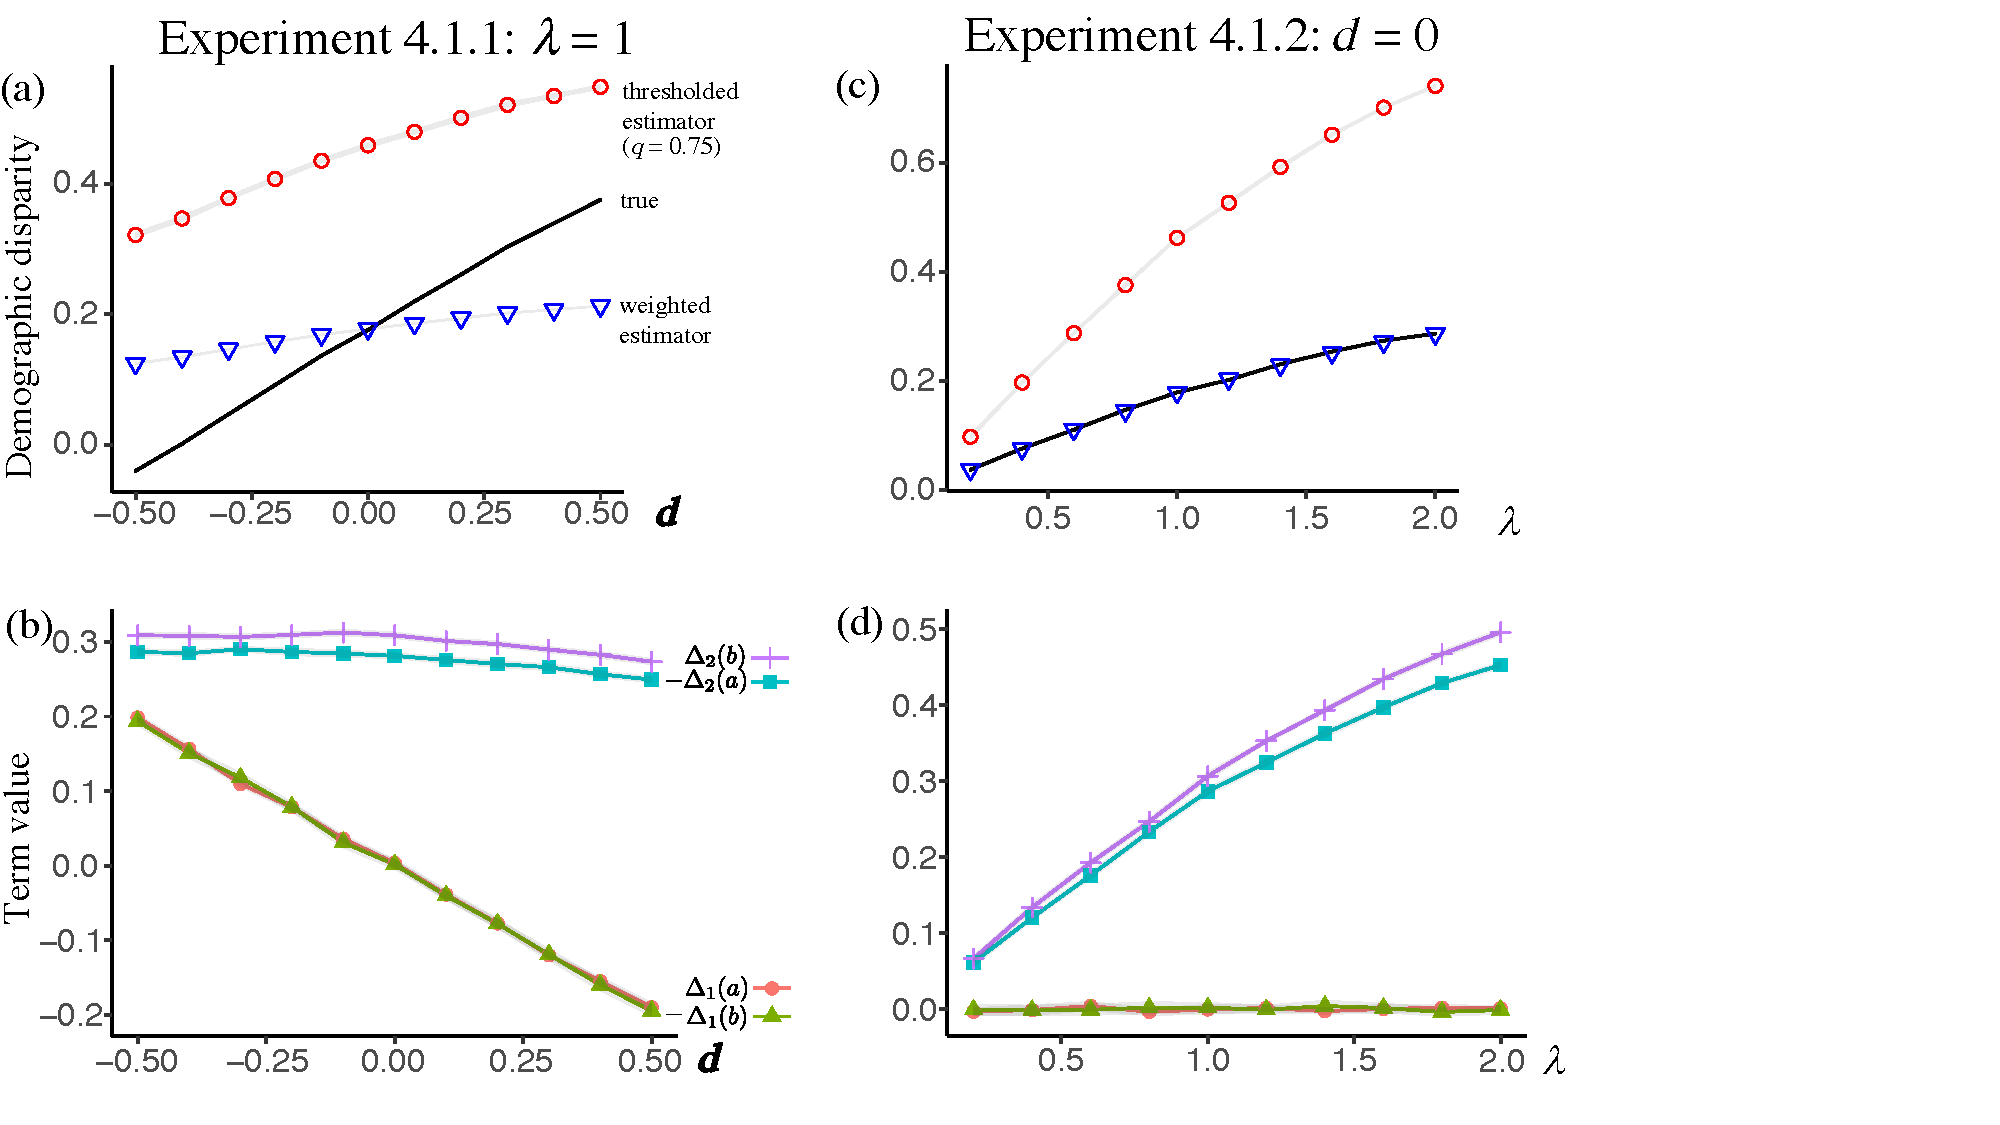
\includegraphics[width = \linewidth]{Simulation.pdf}
\caption{Top row: performance of the thresholded ($\hat{\delta}_{q=0.75}$, red circles) and weighted ($\hat{\delta}_W$, blue triangles) estimators of demographic disparity in Experiments \ref{exp:intra} (a) and \ref{exp:inter} (c), relative to the true demographic disparity (black line).
Bottom row: values of the terms $\Delta_1(a)$, $-\Delta_1(b)$, $\Delta_2(a)$, and $-\Delta_2(b)$ in Corollary \ref{corollary: demographic-est-race} in Experiments \ref{exp:intra} (b) and \ref{exp:inter} (d), showing their contributions to the bias.
Shown in light gray is the confidence interval within two standard deviations,
averaged over 30 simulations, which in all cases is comparable to the width of the plotted lines.
}\label{figure: synthetic}
\end{figure}



Figure \ref{figure: synthetic}(b) shows that in Experiment \ref{exp:intra}, only $\Delta_1\!(a)$ and $\Delta_1\!(b)$ vary strongly with $d$, so they are largely responsible for the bias observed in Figure \ref{figure: synthetic}(a).
When $d < 0$, the disadvantaged group have comparatively higher incomes and are thus more likely to be approved in loan application.
This implies that conditions \eqref{eq:condition1}---\eqref{eq:condition2} hold and therefore result in overestimation bias for the thresholded estimator.
Furthermore, $Y$ covaries negatively with $\ind(A=a)$ and positively with $\ind(A=b)$ conditionally on $Z$, also resulting in an overestimation bias for the weighted estimator.
When $d > 0$, however, conditions \eqref{eq:condition1}---\eqref{eq:condition2} are violated.
The terms $\Delta_1(a)$ and $\Delta_1(b)$ start to counteract overestimation bias, thus the overestimation bias decreases with $d$.
Furthermore, $Y$ now covaries positively with $\ind(A=a)$ and negatively with $\ind(A=b)$, also resulting in an underestimation bias for the weighted estimator.

Figure \ref{figure: synthetic}(d) shows that in Experiment \ref{exp:inter}, only the terms $\Delta_2(a)$ and $\Delta_2(b)$ vary strongly with $\lambda$, so these terms are responsible for the variation observed in the thresholded estimator $\hat\delta_q$ in Figure \ref{figure: synthetic}(c).
As $\lambda$ increases, both $-\Delta_2(a)$ and $\Delta_2(b) > 0$ increase, along with the overestimation bias of $\hat\delta_q$.
In contrast, the weighted estimator $\hat\delta_W$ is unbiased because the income distribution does not depend on race, and so $Y$ is independent with $\ind(A = a)$ and $\ind(A=b)$ conditionally on $Z$.

While presented only for the particular choices of $\lambda=1$ for Experiment \ref{exp:intra} and $d=0$ for Experiment \ref{exp:inter}, the observation of which terms vary strongly with $d$ and $\lambda$ hold true for quite a few different choices.


\subsection{Estimation biases in the HMDA mortgage data set with geolocation proxy for race}
\label{sec:mortgage}

In this section, we use the public HMDA (Home Mortgage Disclosure Act) data set\footnote{Data link: \url{https://www.consumerfinance.gov/data-research/hmda/explore}.} to demonstrate demographic disparity estimation bias when using a probabilistic proxy for race.
This data set contains mortgage loan application records in the U.S.\ for which the geolocation (state, county, and census tract), self-reported race/\-ethnicity, and loan origination outcome were reported, and
has been used in the literature to evaluate the BISG race proxy \cite{Baines:2014aa, CFPB:proxy2014, zhang2016assessing}.
We use the loan data for the years 2011---2012, consistent with \cite{CFPB:proxy2014}.
We denote ${Y} = 1$ if a loan application was approved or originated, and ${Y} = 0$ if it was denied. The final sample contains around 17 million observations with non-missing geolocation, race, and loan origination outcome information.

We consider a race proxy based only on geolocation, as the public data set is anonymized and omits surnames.
This proxy is derived from the racial and ethnic composition of the U.S.\ population that is over 18 years of age,
using the census tracts of the 2010 decennial census\footnote{We use the census tract level geolocation-only proxy constructed by the CFPB, as described in \url{https://github.com/cfpb/proxy-methodology}.}.
For example, the proportion of Hispanic, white, black, and API (Asian or Pacific Islander) in census tract 020100, Autauga County, Alabama are 0.02, 0.86, 0.10, 0.01 respectively, according to the 2010 census.
This quadruple is assigned to all applicants from this census tract as their race proxy.
This probabilistic proxy, while different from BISG, is nevertheless sufficient to demonstrate the general result regarding disparity estimation bias in Section \ref{sec:theorems}.
We present results for Hispanic, white, and black subpopulations in this section, and defer the result for API to the Appendix.



\begin{figure}
\centering
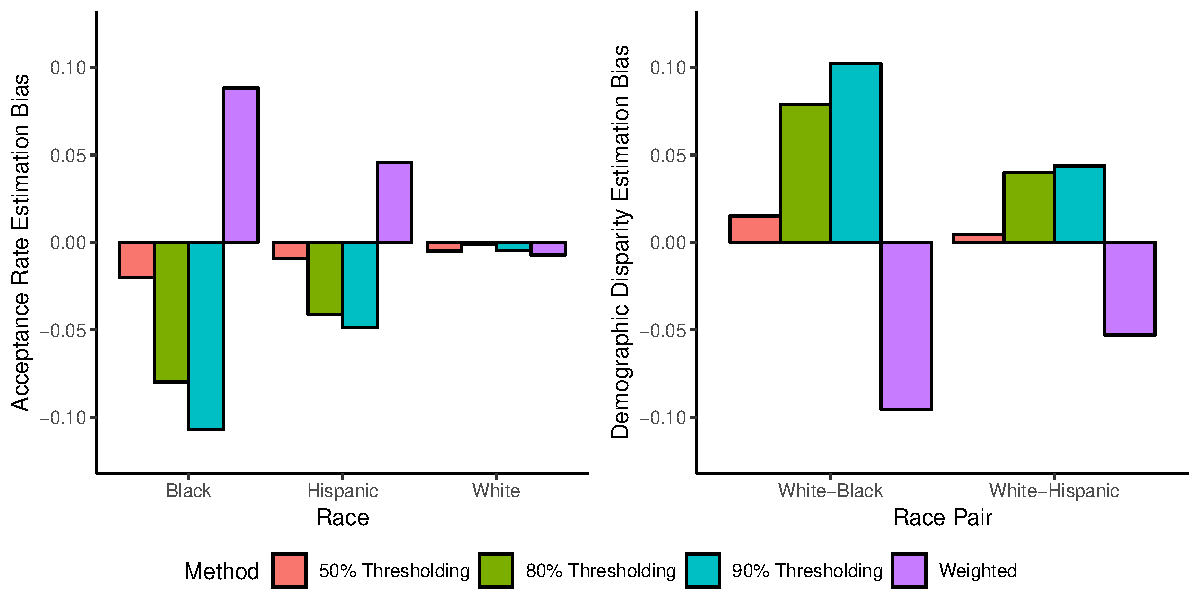
\includegraphics[width=\linewidth]{Demo_disparity_noAPI.pdf}
\caption{Left: estimation biases of loan acceptance rates $\mu$ for different races in the HMDA data set of Section \ref{sec:mortgage}, using the thresholded estimator for mean group outcome $\hat\mu_q$ ($q=0.5, 0.8, 0.9$) from Definition \ref{def:thresholded_estimator}, as well as the weighted estimator $\hat\mu_W$ from Definition \ref{def:weighted_estimator}, relative to the true mean group outcome $\mu$ calculated using the actual race labels.
Right: estimation biases of demographic disparity $\delta$ between pairs of races, using the thresholded estimator $\hat\delta_q$ from Definition \ref{def:thresholded_estimator} and weighted estimator $\hat\delta_W$from Definition \ref{def:weighted_estimator}, relative to the true demographic disparity $\delta$ calculated using the actual race labels.}\label{figure: mortgage_demo_disparity}
\end{figure}

\paragraph{Estimation bias of thresholded estimator and weighted estimator}
In Figure \ref{figure: mortgage_demo_disparity}, we show the estimation bias of the thresholded estimator with different thresholds and the weighted estimator.
Clearly the thresholded estimator underestimates the loan acceptance rate of black and Hispanic groups but it estimates the loan acceptance rate for White group accurately.
As a result, the thresholded estimator overestimates the demographic disparity.
Moreover, the overestimation bias tends to decrease as the threshold $q$ decreases.
In contrast, the weighted estimator displays the opposite performance and underestimates the demographic disparity.

\begin{figure}
\centering
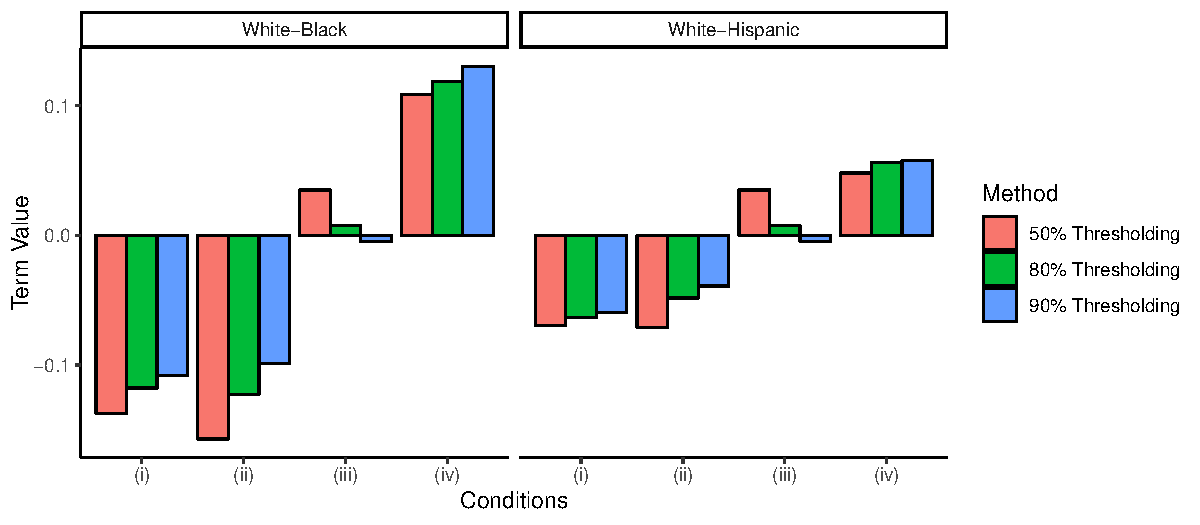
\includegraphics[width=\linewidth]{Demo_condition_noAPI.pdf}
\caption{The values of the terms $\Delta_1(a)$, $-\Delta_1(b)$, $\Delta_2(a)$, and $-\Delta_2(b)$ in Corollary \ref{corollary: demographic-est-race} for the mortgage data set of Section \ref{sec:mortgage}, for thresholds $q=$ 0.5, 0.8, and 0.9.
Negative values demonstrate partial violation of the conditions of Corollary \ref{corollary: demographic-est-race}.} \label{figure: mortgage_demo_disparity_conditions}
\end{figure}

\begin{figure}
\centering
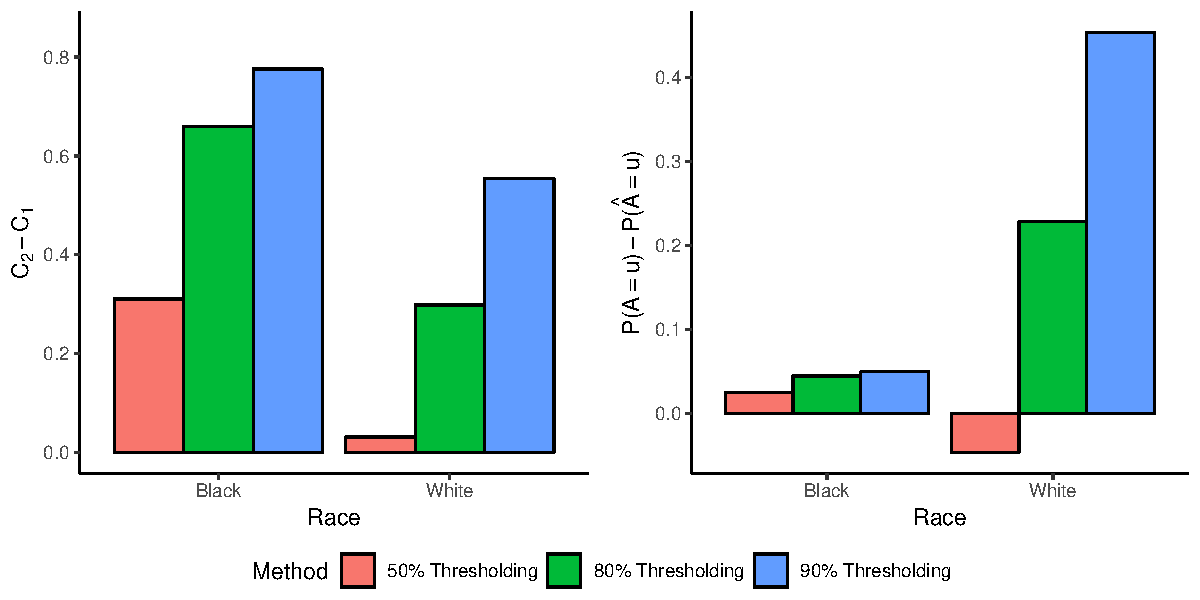
\includegraphics[width=\linewidth]{C_values.pdf}
\caption{Left: the difference between the terms $C_2(u)$ and $C_1(u)$ in Theorem \ref{thm: demographic-est-race-bias} for races $u=$ black or white and thresholds $q=$ 0.5, 0.8 and 0.9 for estimating the race labels according to the thresholded rule of Definition \ref{def:thresholding_rule}.
As $q$ increases, $C_2(u)$ is increasingly larger than $C_1(u)$, and thus the $\Delta_2(u)$ terms contribute more to the estimation bias than the $\Delta_1(u)$ terms.
Right: difference between the probabilities of the true and estimated race labels, $\pr (A = u) - \pr (\hat{A} = u)$. As $q$ increases from 0.5 to 0.9, the proportion of unclassified samples increases from 0.065 to 0.63, which causes $\pr (\hat{A} = u)$ to decrease drastically. As a result, $C_2(u) - C_1(u)$ increases due to Corollary \ref{corollary: C-functions}.}\label{figure: C_values}
\end{figure}
% \footnote{Note that Corollary \ref{corollary: C-functions} assumes binary protected class. The general result is included in Appendix, where $C_2(u) - C_1(u)$ can be positive as long as $\pr (A = u) - \pr (\hat{A} = u)$ is  negative. }


\paragraph{Bias source of thresholded estimator}
Figure \ref{figure: mortgage_demo_disparity_conditions} shows the conditions  \eqref{eq:condition1}---\eqref{eq:condition4}.
Only \eqref{eq:condition4} strictly holds, meaning that people from the disadvantaged group (Hispanic or black) living in census tracts where their race ratio exceeds the corresponding classification threshold have lower average loan acceptance rate than people from the disadvantaged group living in census tracts where their race ratio is not as high as the classification threshold.
This captures the \textit{inter-geolocation} outcome variation: the loan approval is negatively correlated with the disadvantaged group prevalence across the geolocations.
In Example \ref{ex:income}, we give a reason why loan acceptance is correlated with the race proxy probabilities: geolocation is correlated with both race proportions (i.e., race proxy probabilities) and socioeconomic status (e.g., income, FICO score, etc.) that affects loan approval. In Appendix \ref{section:correlation_income}, we validate that such correlations are indeed obvious in the mortgage data set.

In contrast to conditions \eqref{eq:condition4}, conditions \eqref{eq:condition1}---\eqref{eq:condition2} are strictly violated, and condition \eqref{eq:condition3} is slightly violated.
However, the thresholded estimators still have overestimation bias because \eqref{eq:condition3}---\eqref{eq:condition4} have dominant effects, as shown in Figure \ref{figure: C_values}.
Moreover, as the threshold $q$ increases, conditions \eqref{eq:condition3}---\eqref{eq:condition4} start to dominate, increasing the overestimation bias.
Nevertheless, the apparent reduction of overestimation bias when using lower threshold does not mean that using lower threshold is better in practice. Instead, the reduction of overestimation bias is the consequence of delicate counterbalance between the two opposing bias sources: the violation of conditions \eqref{eq:condition1}---\eqref{eq:condition2} contributes to underestimation bias and the conditions \eqref{eq:condition3}---\eqref{eq:condition4} contribute to overestimation bias. Thus, the smaller bias from using a lower threshold is not a robust finding. For example, for the experiments in Section \ref{sec:numerics}, changing the threshold from $0.75$ to $0.5$ does not affect either the race imputation result or the demographic disparity estimation bias. This reflects the intrinsic complexity of the thresholded estimator.

In summary, according to Corollary \ref{corollary: C-functions}, the fact that the thresholded estimation rule for race excludes many unclassified examples makes the overestimation predominantly be determined by the inter-geolocation outcome variation captured by conditions \eqref{eq:condition3}---\eqref{eq:condition4}, especially when the threshold $q$ is very high. Moreover, strong racial segregation and socioeconomic status disparities across different geolocations make condition \eqref{eq:condition3} or \eqref{eq:condition4} (if not both) very likely to hold. As a result, the thresholded estimator tends to overestimate the demographic disparity, especially when high threshold is used. Since BISG also uses geolocation for race estimation, the reported overestimation bias of using thresholded estimator with BISG should be at least largely (if not all) due to the same reason. Moreover, the estimation bias of thresholded can be very sensitive to the threshold value because the threshold value influences the interplay of the bias sources in \eqref{eq:condition1}---\eqref{eq:condition4}. This reflects the intrinsic limitation of the thresholded estimator.


% The strong effect of condition \ref{corollary: demographic-est-race}(iv) clearly shows that the thresholded estimator is likely to be biased when the proxy method is based on predictor that is strongly correlated with the outcome.
% In Example \ref{ex:income}, we present a hypothetical case where geolocation is correlated with both race composition and socioeconomic status.
% Since lending outcome is arguably correlated with socioeconomic status, \textit{the outcome is correlated with the probabilistic proxy} in such a way that the thresholded estimator overestimates the demographic disparity. Although in reality the correlation between the probabilistic proxy and the outcome (and socioeconomic status) is not as extreme as the hypothetical example, we show in the Appendix that the correlations are still apparent. Since the BISG method also uses geolocation information, the overestimation bias should partly (if not all) be caused by  at least one of conditions \ref{corollary: demographic-est-race}(iii)-(iv) that capture the correlation between the outcome and the probabilistic proxy (very likely through socioeconomic status).

\begin{figure}
  \centering
    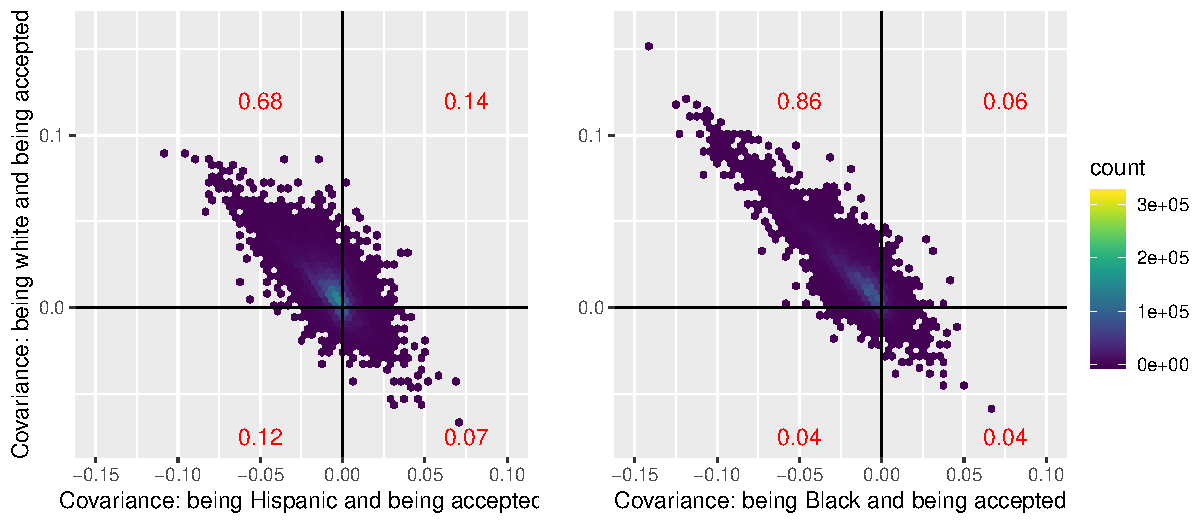
\includegraphics[width=\linewidth]{Weighted_condition_noAPI.pdf}
  \caption{The population distribution across different combinations of within-census-tract-covariances between the loan acceptance and the membership to advantaged group or the membership to disadvantaged group. The red numbers in each quadrant represents the proportion of people who live in census tracts with the corresponding covariance combination.} \label{figure: mortgage_weighted_conditions}
\end{figure}

\paragraph{Bias source of the weighted estimator}
Figure \ref{figure: mortgage_weighted_conditions} shows the distribution of population who live in census tracts with different combinations of $\cov (\ind(A = a), {Y} \mid Z)$ and $\cov (\ind(A = b), {Y} \mid Z)$ with $a$ representing white and $b$ representing black or Hispanic.
Theorem \ref{thm: weighted} implies that the upper left quadrants account for the underestimation bias of weighted estimator for demographic disparity,
as these quadrants contain all census tracts where the loan acceptance is positively correlated with membership to the advantaged group ($\cov (\ind(A = a), {Y} \mid Z) > 0$),
while negatively correlated with the membership to the disadvantaged group ($\cov (\ind(A = b), {Y} \mid Z) < 0$).
Figure \ref{figure: mortgage_weighted_conditions} shows that the majority of people live in census tracts falling in the upper left quadrants.
In other words, most people live in census tracts where white people have a higher average loan approval rate than their black or Hispanic neighbors. This explains the underestimation bias of the weighted estimator since the estimation bias of the weighted estimator is solely determined by the intra-geolocation outcome variation according to Theorem \ref{thm: weighted}.

% This explains the overall underestimation bias of the weighted estimator. Plus, since conditions \ref{corollary: demographic-est-race}(i)-(ii) are closely related to the estimation bias of the weighted estimator according to Proposition \ref{prop: relation-weighted-thresholding}, the population concentration in the upper left quadrants also explains why conditions \ref{corollary: demographic-est-race}(i)-(ii) are strictly violated.


\paragraph{Summary}
The empirical results show that our theoretical analysis provides convincing explanations for the observed estimation bias of the thresholded estimator and the weighted estimator. We show that the bias sources of the weighted estimator and the thresholded estimator are very different: the bias of the weighted estimator is solely determined by the intra-geolocation variation, and the bias of the thresholded estimator is determined by both inter-geolocation variation and intra-geolocation variation. When high threshold is used, the inter-geolocation variation dominates.
In the mortgage dataset, we show that the racial segregation, socioeconomic status, outcome disparity pattern with respect to geolocation make the thresholded estimator tend to overestimate the demographic disparity, and the weighted estimator tend to underestimate the demographic disparity.
This explains the overestimation bias of the thresholded estimator with BISG reported by previous literature.
Moreover, our results show that the estimation bias of thresholded estimator is sensitive to the threshold because of complex interplay of different bias sources.
As a result, the observed estimation bias pattern in one setting may hardly generalize to other settings.
In contrast, the weighted estimator only has one bias source, and is thus easier to reason about. 

% On the one hand, our empirical results show that the thresholded estimator tends to overestimate demographic disparity and the weighted estimator tends to underestimate demographic disparity. Therefore, using both together can hopefully bracket the true demographic disparity. On the other hand, we also show an example that after explicitly considering our theoretical results, it is possible to construct a proxy model that leads to accurate estimation of demographic disparity.


%  \ref{thm: demographic-est-race} hold in practice and if the conditions explain the observed bias in estimating the disparate impact.

% Plan:
% \begin{enumerate}
% \item Use geolocation only method to construct race probabilities and use a table to compare the demographic disparity using true race, estimated race under thresholding rule, weighted estimator.
% \item Evaluate the correlation between $\hat{Y}$ and $\pr (A = a \mid Z)$ for different a (white, black, Asian, Hispanic):
%   \begin{enumerate}
%     \item Box plot: $\pr (A = a \mid Z)$ against $Y = 0, 1$; this evaluates condition (a)(b);
%     \item Bar plot: Acceptance rate corresponding to $A = w, b$ conditionally on $\pr (A = w \mid Z) > t$ and $\pr (A = b \mid Z) > t$; this evaluates condition (c)(d)
%     \item Evaluate if the most ambiguous census tract also has the intermediate values of acceptance rate (not very high nor very low)
%   \end{enumerate}
% \item We can possibly condition on the loan type to evaluate the conditional demographic disparity
% \end{enumerate}
